% MUST use a4paper option
% MAY use twoside, smaller font, and other class - but not for Självständigt arbete i IT
\documentclass[a4paper,12pt]{article}
% Use UTF-8 encoding in input files
\usepackage[utf8]{inputenc}
% Use T1 font encoding to make the \hyphenation command work with UTF-8
\usepackage[T1]{fontenc}

% Om ni skriver på svenska, använd denna rad:
% \usepackage[english,swedish]{babel}
% If you are writing in English, use the following line INSTEAD of the previous (note order of parameters):
\usepackage[swedish,english]{babel}

% Use the template for thesis reports
\usepackage{UppsalaExjobb}

\usepackage{enumitem}
\usepackage{svg}
\usepackage{subcaption}
\usepackage{caption}
\usepackage{mwe}

% För att göra ett index behövs
%  - \usepackage{makeidx}
%  - \makeindex i "preamble", dvs före \begin{document}
%  - \printindex, typiskt sist, före \end{document}
% - och att man lägger in \index{ord} på olika ställen i dokumentet
\usepackage{makeidx}
\makeindex


% Designval: per default används styckesindrag, men ibland blir det snyggare/mer lättläst med tomrad mellan stycken. Det åstadkoms av de följande raderna.
% Tycker ni om styckesindrag mera, kommentera bort nästa två rader.
\parskip=0.8em
\parindent=0mm

% Designval: vill ni ha en box runt figurer istället för strecken som är default, av-kommentera raden nedan. Obs att både \floatstyle och \restylefloat behövs.
%\floatstyle{boxed} \restylefloat{figure}

\begin{document}
% För att ställa in parametrar till IEEEtranS/IEEEtranSA behöver detta ligga här (före första \cite).
% Se se IEEEtran/bibtex/IEEEtran_bst_HOWTO.pdf, avsnitt VII, eller sista biten av IEEEtran/bibtex/IEEEexample.bib.
%%%% OBS: här ställer ni t.ex. in hur URLer ska beskrivas.
\bstctlcite{rapport:BSTcontrol}

% Set title, and subtitle if you have one
\title{Allocators in OpenJDK} % och uppsatsmetodik
% Use this if you have a subtitle
%\subtitle{beskrivande men gärna lockande}
%\subtitlesubtitle

% Set author names, separated by "\\ " (don't forget the space, or use newline)
% List authors alphabetically by LAST NAME (unless someone did significantly more/less, which should not be the case)
% For drafts, include your email addresses to make it easier to send peer reviews
\author{Casper Norrbin}

% Visa datum på svenska på förstasidan, även om ni skriver på engelska!
\date{\begin{otherlanguage}{swedish}  %\foreignlanguage doesn't seem to affect \today?
    Juni 2024
  \end{otherlanguage}}

% Använd detta om året för rapporten inte är innevarande år
%\year=2018

% Ange handledare, ämnesgranskare, examinator om dessa finns
\handledare{Erik Österlund}
% There is also \exthandledare
\reviewer{Tobias Wrigstad}
\examinator{Lars-Åke Nordén}

% This creates the title page
\maketitle

% Change to frontmatter style (e.g. roman page numbers)
\frontmatter

%%%% OBS: Läs också källkoden till alla text/X.tex.
%%%% Tips: ni kan använda separata filer för de olika delarna i er rapport på motsvarande sätt,
%%%% men använd inte samma filnamn!

\begin{abstract}
  
%%% Local Variables:
%%% mode: latex
%%% TeX-master: "main"
%%% End:
Memory fragmentation is a common issue in programs running with dynamic memory allocations. Java is a programming language that solves the problem of memory fragmentation by using garbage collectors. The most recent garbage collector added to Java, ZGC, solves fragmentation by moving objects around in memory, leading to more densely packed allocations. ZGC performs sequential allocations with the use of a bump-pointer, which offers great execution times, but has the issue of causing fragmentation due to its inability to reach certain areas of free memory.

This thesis present a new solution to compacting memory in ZGC using free-list based allocators. By using free-lists to represent the fragmented memory as available space, allocations can utilize the previously considered unreachable memory as a target location for compaction. The trade-off of introducing this new allocation strategy is a more computationally heavy allocation method, but more total memory that can be utilized for compaction. Results from this thesis show promising results when utilizing an optimized version of a TLSF allocator, showing good possibilities of moving objects into fragmented memory.


% in programs that run for longer periods of time. By continuously alternating between allocating and releasing memory, the program can cause the memory to become fragmented, meaning objects are no longer stored in a contiguous block of memory. The free regions of memory between objects can then be hard to utilize, because certain objects might not fit in that space. In programming language with dynamic memory management, this issue can be solved by a garbage collector which automatically frees up memory that is no longer in use. Different garbage collectors have different strategies for managing memory, but they all aim to reduce fragmentation and improve the performance of the program. In this thesis, we will explore the use of free-list allocators in garbage collectors, and its integration in one of Java's latest garbage collectors, ZGC. ZGC uses bump pointers to allocate memory which allows for fast allocations. However, it is known that bump pointers can cause fragmentation in the memory. The goal of using a free-list allocator is to let the garbage collector know that there is free space available in between allocations, which is something that bump pointers are not able to do. We will investigate the feasibility of using such an allocator and how it can be used to compact memory.


\end{abstract}

\begin{sammanfattning}
  
%%% Local Variables:
%%% mode: latex
%%% TeX-master: "main"
%%% End:

\end{sammanfattning}

% Innehållsförteckningen här.
\tableofcontents

% Här kan man också ha \listoffigures, \listoftables

\cleardoublepage

% Change to main matter style (arabic page numbers, reset page numbers)
\mainmatter

% Here comes the text of the report.

\section{Introduction}
\label{sec:introduction}

%%% Local Variables:
%%% mode: latex
%%% TeX-master: "main"
%%% End:
%The goal of this thesis project is to investigate the possibility of using free-list allocators in garbage collectors. The project will focus on integrating a free-list allocator in the ZGC, a garbage collector available in the most recent release of the OpenJDK. Currently in ZGC, memory is allocated in regions using sequential allocators, discussed in more detail in Section~\ref{sec:background}. Although it is a very performance effective way of allocating objects, it is known that bump pointers can cause a lot of external fragmentation in the memory~\cite{TODO:bump}. By making use of a free-list allocator, it is possible to let the garbage collector know that there is free space available in between allocations, allowing for allocations inside of the externally fragmented memory. This will add some extra work load on the allocation of objects, but will allow for using memory more efficiently. The project will investigate the feasibility of using such an allocator, and whether it improves the throughput and or memory usage.
Garbage collection is a feature in many dynamical programming languages, where the task of a garbage collector is to keep track of which parts in the memory is currently being used by the running program. Efficient memory management is useful for increasing the performance and resource usage of programs, since all of the memory utilization is heavily relying on how the memory is being kept track of by the underlying garbage collector.

Java is a dynamical programming language that makes use of garbage collectors in order to handle memory. Java is used by one of the largest services on Earth, Netflix. Operating within a runtime environment known as the Java Virtual Machine (JVM), Java allows users to configure the JVM for optimal performance, including the choice of garbage collector. In Mars 2024, a blogpost from Netflix was released~\cite{netflix:zgc}, announcing the benefits of switching from one garbage collector, to the latest, most modern garbage collector, generational ZGC. They found that the upgrade yielded an improvement of 6-8\% percent in CPU utilization, proving that new technologies can lead to great improvements.

This thesis will continue on the subject of further exploring possible improvements that can be made to the JVM and its garbage collectors. Specifically, the goal is to look at lowering the amount of memory used by ZGC by using new methods of allocating objects in fragmented parts of memory. 

\subsection{Purpose and Goals}
\label{sec:purpose}
The main goal of this project is to explore how free-list allocators can be integrated into compacting garbage collectors. Specifically, we'll focus on adding a free-list allocator into the Z Garbage Collector (ZGC) in the latest version of OpenJDK. Currently, ZGC uses sequential allocators to manage memory allocation in regions (explained further in Section~\ref{sec:background}). While this method is quick when allocating objects, it struggles with external fragmentation due to the nature of bump pointers, which is talked about in more detail in Seciton~\cite{background:memorymanagement}. By introducing a free-list allocator, we aim to inform the garbage collector about available free space between allocations, improving memory usage within fragmented regions. Although this increases the workload for allocating objects, it opens up the possibility of compacting memory in a new way.

This project will evaluate the feasibility of integrating a free-list allocator into ZGC and evaluate its impact on throughput and memory usage. Through this investigation, we aim to contribute to improving garbage collection techniques, potentially leading to more efficient memory management in the JVM.
%%% Local Variables:
%%% mode: latex
%%% TeX-master: "main"
%%% End:


\subsection{Delimitations}
\label{sec:delimitations}
%%% Local Variables:
%%% mode: latex
%%% TeX-master: "main"
%%% End:
This report will only cover the integration of a free list allocator in ZGC, and not the implementation of the allocator itself. The integration process will assume that such an allocator is already available, and the project will focus on integrating it into the ZGC code base.

As this project will cover the integration of a free list allocator in a large code base, the project will be limited to using the free list allocator in the specific case of relocating objects in ZGC. Relocation is a big part of ZGC, and is the method used for compacting memory. The allocator could potentially be used in other areas of the JVM, but this thesis will focus on the impact it has on the memory compaction of ZGC. This is explained in more detail in Section~\ref{background:relocation}. 

\subsection{Individual Contributions}
\label{sec:individual_contrubitons}

This thesis was written primarily by Niclas Gärds, but Section 2 was coauthored by Joel Sikström and Casper Norrbin. More specifically, section 2.1, 2.2, 2.3 was written by Joel, and 2.4 was written by Casper.


%%% Local Variables:
%%% mode: latex
%%% TeX-master: "main"
%%% End:


\paragraph{Acknowledgement}

%%% Local Variables:
%%% mode: latex
%%% TeX-master: "main"
%%% End:


\newpage
\section{Background}
\label{sec:backgrond}

%%% Local Variables:
%%% mode: latex
%%% TeX-master: "main"
%%% End:


\subsection{Memory Management}
\label{sec:memory_management}

Memory management is typically categorized into being either manual or automatic. Manual memory management involves explicitly assigning and managing memory by the programmer, which is commonly used in low-level languages like C and C++. Automatic memory management is handled automatically by the system, without the need for the programmer to intervene. One method for achieving automatic memory management is through the use of a garbage collector, a mechanism responsible for both allocating and releasing memory. Languages like Python and Java are examples of programming languages that do this.

Memory is most commonly allocated during runtime of the program as opposed to allocating everything in advance, during startup for example. The process of allocating memory during runtime is referred to as dynamic memory management, which presents a number of challenges for reliably being able to satisfy allocation requests and run for extended periods of time.

The main problem with dynamic memory allocation is that an allocation might fail due to memory exhaustion. Exhaustion may arise either due to the program requiring more memory than is available in the system or from the circumstance where free memory is available but cannot be reused. The second case is sometimes referred to as just wasted memory, but to be precise we will classify it as either internal or external fragmentation, which will be discussed further below.

%%% Local Variables:
%%% mode: latex
%%% TeX-master: "main"
%%% End:


\subsection{Fragmentation}
\label{sec:fragmentation}

% Beskriva skillnad mellan internal och external fragmentation och att de kan anses som samma sak, "wasted space" (TLSF paper).

% Kanske fixa två figurer som visar på exakt vad det handlar om (om det är relevant)?

%%% Local Variables:
%%% mode: latex
%%% TeX-master: "main"
%%% End:


\subsection{Memory Allocation}
\label{sec:memory_allocation}

In this section, we describe two fundamental memory allocation strategies, called sequential allocation and free-list allocation~\cite{gchandbook}. Additionally, we discuss the more complex case of using multiple free-lists, called segregated-fits.

\subsubsection{Sequential Allocation}
\label{sec:seq_allocation}
\label{sec:bump_pointer}

Sequential allocation is a method used for allocating memory within a contiguous chunk of memory. In this approach, a pointer is used to track the current position within the memory chunk. As new objects are allocated, the pointer is advanced by the size of the object, along with extra memory that might be needed for alignment purposes. For this reason, sequential allocation is also known as bump-pointer allocation due to the incremental ``bumping'' of the pointer with each new allocation. 

This approach is simple and efficient and is highly effective in situations where memory fragmentation is not a significant concern and where a predictable, sequential layout is desirable. However, it may not be the most suitable choice for all scenarios, especially where memory is not available in a large contiguous chunk. In that case, a more sophisticated memory management strategy might be required. 

\subsubsection{Free-List Allocation}

An alternative to sequential allocation is free-list allocation, which involves maintaining a record of the location and size of available blocks in a linked list, for example. In its simplest form, a single list is used to track free blocks. The allocator then sequentially considers each block and selects one according to a specified policy. Below, we will provide an overview of the most common policies used in free-list allocation.

\begin{description}
    \item[First-fit]
        The first block in the free-list that is large enough to fulfill the memory allocation request is selected. This method minimizes search time but does not consider the possibility of a more suitable block elsewhere in the list. This often leads to more fragmentation than is necessary, because blocks are split more often. New requests restart their search from the beginning of the list.
    \item[Next-fit]
        The search for a suitable block begins in the free-list, following a similar process to that described for first-fit. However, in subsequent searches, it resumes from where the previous search ended, improving efficiency when locating a new block. This strategy is based on the observation that smaller blocks tend to accumulate at the beginning of the free-list~\cite{gchandbook}, optimizing the search process by starting further into the list in each iteration.
    \item[Best-fit]
        The entire free-list is searched until the smallest available block that can fulfill a request is located. This method minimizes fragmentation by selecting the block that best matches the size of the requested memory, but it comes with the trade-off of increased search time.
\end{description}

The three policies described above have in common that when a block that is larger than requested is found, it is split up. Blocks are generally desired to be split as infrequently as possible to have larger blocks available for larger requests. If blocks are split too often, many small blocks might accumulate, which might increase external fragmentation to a level where new requests cannot be fulfilled. Additionally, splitting blocks less frequently will also mean less merging, or coalescing, of blocks to larger sizes, which could improve performance.

\subsubsection{Segregated-Fits Allocation}

Instead of using a single free-list where blocks of many sizes are stored, multiple free-lists that store blocks of similar sizes or size ranges can instead be used, called segregated-fits. The goal of using multiple free-lists is to narrow down the search space to fewer blocks, minimizing the time to find blocks large enough to satisfy a request. It is crucial to note that blocks are logically segregated into their respective free-lists based on size but are not required to be physically adjacent in memory within the same free-list. 

Segregated-fits is often employed in real-time systems where predictable and efficient memory allocation is crucial~\cite{gchandbook, TLSF}. The reduced search space and minimized search time to find suitable blocks increase the probability of timing constraints being met.

%%% Local Variables:
%%% mode: latex
%%% TeX-master: "main"
%%% End:


\newpage
\subsection{Garbage Collection}
\label{sec:gc}

This section draws heavily from \textit{The Garbage Collection Handbook: The Art of Automatic Memory Management}~\cite{gchandbook}, by Jones et al., which provides a comprehensive overview of garbage collection methods, both historical and current.

As mentioned in Section~\ref{sec:memory_management}, garbage collection is a form of automatic memory management where the system identifies and cleans up unused objects, which are considered garbage. This removes the requirement of managing memory manually, which reduces the possibility of user-related memory issues occurring. However, this also removes some control from the user and could lead to an increased memory footprint.

From the perspective of the GC, the user program can be perceived solely as a memory mutator. This is because the GC is only concerned with the memory management of the program, not its functionality. Therefore, the threads of the user program are commonly referred to as mutator threads, or just mutators.

During GC execution, it may be necessary to temporarily halt the mutator threads to give the GC exclusive memory access. This is known as a stop-the-world approach. From the mutator's perspective, the GC appears to be atomic. This permits a simple implementation and avoids synchronization between GC and mutators while the GC is running, but also introduces pauses in the application which may be undesirable if latency is a quality metric. The GC could also operate concurrently and in parallel with the mutator threads. This leads to increased complexity as the memory can mutate during GC execution. Most GCs fall somewhere in between these ends, executing concurrently with the mutator threads while occasionally requiring pauses in their execution.

There exist numerous garbage collection strategies. One is the mark-sweep algorithm, which begins by identifying a set of accessible "root" objects. Roots are objects that serve as entry points into the object graph, such as global variables, local variables in stack frames, and registers. Roots are then marked as live and scanned to identify other objects in the object graph. This process continues recursively until all live objects have been identified. Afterwards, the heap is swept, meaning that the space not occupied by live objects is made available for new allocations.

The mark-sweep algorithm does not move objects, which can result in higher levels of external fragmentation. The mark-compact algorithm addresses this issue. Like mark-sweep, it traverses the heap and marks all live objects. However, instead of sweeping, live objects are moved and compacted. This approach reduces fragmentation and can be managed using a simple bump-pointer allocator. 

A copying garbage collector divides the heap into many subheaps. A subheap is first chosen and marked as non-empty. Allocations are then made sequentially onto this subheap using bump-pointer allocation. When garbage collection is initiated, live objects are copied from their current subheap to another subheap. Once all live objects have been copied, the original subheap is marked as empty and its bump-pointer reset. Compared to mark-compact, heap size is significantly reduced when using few subheaps. Using many subheaps will make each subheap small, which could result in more, and likely shorter, garbage collection cycles.

%%% Local Variables:
%%% mode: latex
%%% TeX-master: "main"
%%% End:


\subsection{OpenJDK}
\label{sec:openjdk}

OpenJDK~\cite{openjdk} is a set of tools for creating and running Java programs, maintained by Oracle. HotSpot~\cite{hotspot} is one of these tools and the reference implementation of the Java Virtual Machine (JVM)~\cite{JVM}. Specifically, a virtual machine (VM) emulates a distinct computer to run various programs, which could be anything from full operating systems -- to more specialized machines. The JVM is designed specifically to execute Java programs. It translates programs to instructions for the underlying machine, creating an abstraction of the hardware of the physical machine and allows Java programs to be run on any platform that the JVM runs on.

HotSpot is comprised of several components, such as an interpreter, a Just-In-Time (JIT) compiler, and a garbage collector (GC). In combination, these components provide the means for running different types of Java programs on the platforms supported by HotSpot.

HotSpot provides several garbage collectors, each with different characteristics and performance profiles. Different garbage collectors are optimized for different use cases, such as throughput and latency, and can be tuned to varying degrees. One of the garbage collectors in HotSpot is the Z Garbage Collector (ZGC)~\cite{zgc}. It was introduced as an experimental feature in OpenJDK 11, and declared production ready in OpenJDK 15. ZGC is a modern, generational, region-based, concurrent garbage collector that aims to keep pause times constant at any given heap size.

%%% Local Variables:
%%% mode: latex
%%% TeX-master: "main"
%%% End:



\subsection{The Z Garbage Collector}
\label{sec:zgc}

ZGC is a garbage collector available in the OpenJDK. It was introduced as an experimental feature in OpenJDK 11, and declared production ready in OpenJDK 15. ZGC is modern, generational, region-based, concurrent garbage collector that aims to keep pause times constant at any given heap size. This means latency will remain low as the heap size increases.

The following sections will cover the basics of how ZGC allocates data and how it is able to dynamically collect garbage. The information is based partly on an overview by A. M. Yang and T. Wrigstad~\cite{zgc:deep_dive} and partly on the source code of ZGC itself, as available in OpenJDK version 22.32~\cite{jdk:tag2232}.

%%% Local Variables:
%%% mode: latex
%%% TeX-master: "main"
%%% End:


\subsubsection{Pages}
\label{sec:zpage}

ZGC is a region-based garbage collector which allocates objects inside units of memory that are referred to as pages. New objects are allocated inside pages with respect to their size. Pages are classified as one of the three different types: \textit{Small}, \textit{Medium} or \textit{Large}, which support allocations of different size ranges, as specified in Table~\ref{table:zpage_sizes}. All allocations are aligned to 8 bytes and the smallest supported allocation size is, at the time of writing, 16 bytes. As a result of all allocations having the same alignment, their offset from the start of the page will also be a multiple of the alignment.

\begin{table}[H]
    \centering
    \begin{tabular}{lllll}
        Page Type   & Page Size     & \multicolumn{3}{l}{Object Size}      \\ \hline
        Small       & 2 MB          & \multicolumn{3}{l}{{[}16B, 256KB{]}} \\
        Medium      & 32 MB         & \multicolumn{3}{l}{(256KB, 4MB)}     \\
        Large       & $\geq$ 4 MB   & \multicolumn{3}{l}{$\geq$ 4MB}       \\
    \end{tabular}
    \caption{Page sizes in ZGC. (Figure taken from~\cite{zpage_size_table}). }
    \label{table:zpage_sizes}
\end{table}

Pages in ZGC keep track of information that allow them to efficiently allocate new memory and work concurrently with multiple threads. An overview of this information is shown in Figure~\ref{fig:zpages}, where the most important attributes are the: \textit{Bump Pointer}, \textit{Live Map}, \textit{Sequence Number}, and \textit{Age}, which are explained in detail below.

\begin{description}
    \item[Bump Pointer]
        The bump pointer points to the location where new allocations are made inside the page. Its functionality and use-case is explained in greated detail in Section~\ref{sec:bump_pointer}. All allocations inside pages in ZGC are currently done using bump pointers.

    \item[Live Map]
        The live map is used to keep track of which objects are currently live and have been marked as reachable by the program. Objects not marked in the live map are considered dead and can be reclaimed by the GC. The live map is illustrated on the right-hand side of Figure~\ref{fig:zpages}. It is constructed during the marking phase of the GC cycle as live objects are encountered during memory traversal and stored in a bitmap. Each bit is mapped to an 8 byte chunk of the page and if a bit is set, there is a live object at the corresponding place in the page. The data collected in the live map is later used during the compacting phase, which will contain knowledge about what objects can be reclaimed.

        \newpage
    \item[Sequence Number]
        Every page has a sequence number denoting during which GC cycle it was created. New allocations are exclusively done in pages created after the latest GC cycle. Pages which created before the current GC cycle are therefore separated from new ones, allowing the GC to work concurrently while the program is executing. For example, if the current Java program has performed 5 GC cycles, any allocations after that will be exclusively done on pages with sequence number 5. If the program decides to run a 6th cycle, only garbage from pages with sequence number 0 through 5 will be collected, and new allocations are done on pages with sequence number 6.

    \item[Age]
        ZGC is a generational garbage collector, meaning it treats objects of varying age differently to improve performance. This is based on the observation that most objects survive for only a short period of time and those that survive for longer tend to live for a long time. ZGC applies this approach on a page-by-page basis, where all allocations on a page share the same age, which is conveniently stored on each page instead for every object. Objects are grouped into three different age categories: \textit{Eden}, \textit{Survivor} and \textit{Old}. The \textit{Eden} age is for first-time allocation, \textit{Survivor} signifies objects that have survived one or more GC cycles and \textit{Old} those that have survived a threshold of cycles in the \textit{Survivor} age. Classifying pages this way allows the GC to treat pages of a certain age differently, which is especially useful for \textit{Eden} pages, which tend to accumulate garbage quickly.
\end{description}

\begin{figure}[H]
    \centering
    \includesvg[scale=0.8]{figures/zpage_withage.svg}
    \caption{Illustration of a page in ZGC showing what kind of metadata is kept track of to facilitate allocation and object bookkeeping. The page contains three live objects marked in green and with the corresponding bit set in the live map to the right.} 
    \label{fig:zpages}
\end{figure}

\subsubsection{The Garbage Collection Cycle}

Figure~\ref{fig:zgc_timeline} shows a timeline of a garbage collection cycle in ZGC, made up of an example heap and pages. The timeline shows the different phases of a cycle and how the garbage collector prepares for relocating memory to free unused memory. The three different steps in the timeline show:

\vspace*{-0.4cm}

\begin{enumerate}[label=\alph*)]
    \item The initial state of the heap before the first GC cycle. The left page has about 30\% free memory and the right page has about 50\%. The current cycle is 1, as shown by the digit on the top left of each page.
    \item The GC cycle has started, and the old pages have been frozen. New allocations are now done on new pages instead of old ones. The old pages that have been frozen are blue and new pages containing a sequence number are gray.
    \item The GC has finished the marking phase and now have liveness data that indicate where live objects are allocated inside pages.
\end{enumerate}

\vspace*{-0.4cm}

\begin{figure}[H]
    \centering
    \begin{subfigure}[t]{.214\textwidth}
        \centering
        \includesvg[width=1\textwidth]{figures/zrel1.svg}
        \caption{Initial state of the heap before the first GC cycle.}
        \label{fig:zrel1}
    \end{subfigure}
    \hfill\vline\hfill
    \begin{subfigure}[t]{.32\textwidth}
        \centering
        \includesvg[width=1\textwidth]{figures/zrel2.svg}
        \caption{The state of the heap after marking has started.}
        \label{fig:zrel2}
    \end{subfigure}
    \hfill\vline\hfill
    \begin{subfigure}[t]{.32\textwidth}
        \centering
        \includesvg[width=1\textwidth]{figures/zrel3.svg}
        \caption{The state of the heap after all live objects are marked.}
        \label{fig:zrel3}
    \end{subfigure}
    \caption{Timeline of a garbage collection cycle, showing the state of the heap in the different phases.}
    \label{fig:zgc_timeline}
\end{figure}

\vspace*{-0.49cm}

ZGC frees memory marked as garbage by copying live objects from one page to another and re-purposing the source page for new allocations. This leads to the fragmented layout of allocated memory to be compacted which makes it possible to fit objects from multiple pages into a single one. The process of copying live objects is referred to as relocation. When performing relocation, there are two different scenarios that can occur. The first scenario, where a successful relocation is done by copying items to a new page, is illustrated in Figure~\ref{fig:zrel_new}. This type of relocation requires the heap to have enough free space available to create a new page during the time of relocation. Figure~\ref*{fig:zrel_new1} shows a newly created page, and in Figure~\ref*{fig:zrel_new3}, the old page is freed from memory. The total amount of memory is not decreased, but results in a compacted layout with minimal fragmentation.

\begin{figure}[H]
    \centering
    \begin{subfigure}[t]{.2\textwidth}
        \centering
        \includesvg[width=1\textwidth,height=1.2885\textwidth]{figures/zrel_new1.svg}
        \caption{A page has been selected for relocation due to high fragmentation.}
        \label{fig:zrel_new1}
    \end{subfigure}
    \hfill\vline\hfill
    \begin{subfigure}[t]{.2\textwidth}
        \centering
        \includesvg[width=1\textwidth]{figures/zrel_new2.svg}
        \caption{A new page is created with a new sequence number that is used as a relocation target.}
        \label{fig:zrel_new2}
    \end{subfigure}
    \hfill\vline\hfill
    \begin{subfigure}[t]{.2\textwidth}
        \centering
        \includesvg[width=1\textwidth]{figures/zrel_new3.svg}
        \caption{The objects from the first page are relocated to the new page.}
        \label{fig:zrel_new3}
    \end{subfigure}
    \hfill\vline\hfill
    \begin{subfigure}[t]{.2\textwidth}
        \centering
        \includesvg[width=1\textwidth]{figures/zrel_new4}
        \caption{All objects have been copied to the new page and the old page is re-purposed.}
        \label{fig:zrel_new3}
    \end{subfigure}
    \caption{An example of how a successful relocation is done when the heap has enough space to allocate a new page.}
    \label{fig:zrel_new}
\end{figure}

In the previous example, relocation was successful in allocating a new page to relocate objects into. If the heap does not have enough space for a new page, the GC will instead resort to performing an in-place compaction. An in-place compaction is an expensive operation re-arranges the objects of a page without a separate page as a destination. It requires the thread performing the re-arrangement to write to the memory of the page while other threads may read its contents. To do this safely, any threads trying to read from the page during this process must be paused, which removes concurrent execution of the page. The process of in-place compaction of a page is illustrated in Figure~\ref{fig:zrel_in}.

\begin{figure}[H]
    \centering
    \begin{subfigure}[t]{.2\textwidth}
        \centering
        \includesvg[width=1\textwidth,height=1.2885\textwidth]{figures/zrel_in1.svg}
        \caption{The first live object in the page is moved to the start of the page.}
        \label{fig:zrel_in1}
    \end{subfigure}
    \hfill\vline\hfill
    \begin{subfigure}[t]{.2\textwidth}
        \centering
        \includesvg[width=1\textwidth,height=1.2885\textwidth]{figures/zrel_in2.svg}
        \caption{The second live objects is moved as close to the start as possible.}
        \label{fig:zrel_in1}
    \end{subfigure}
    \hfill\vline\hfill
    \begin{subfigure}[t]{.2\textwidth}
        \centering
        \includesvg[width=1\textwidth,height=1.2885\textwidth]{figures/zrel_in3.svg}
        \caption{All objects have been moved, and the space after is made available.}
        \label{fig:zrel_in1}
    \end{subfigure}
    \hfill\vline\hfill
    \begin{subfigure}[t]{.2\textwidth}
        \centering
        \includesvg[width=1\textwidth,height=1.2885\textwidth]{figures/zrel_in4.svg}
        \caption{The bump pointer is moved to the beginning of available space.}
        \label{fig:zrel_in1}
    \end{subfigure}
    \caption{An example of how in-place compaction is done to remove fragmentation.}
    \label{fig:zrel_in}
\end{figure}
 
%%% Local Variables:
%%% mode: latex
%%% TeX-master: "main"
%%% End:


\section{Related work}

%%% Local Variables:
%%% mode: latex
%%% TeX-master: "main"
%%% End:


\section{Theory}
\label{sec:theory}

%%% Local Variables:
%%% mode: latex
%%% TeX-master: "main"
%%% End:

This section continues on the topic of different allocation methods presented in Section~\ref{sec:background}(TODO 2.2?). Depending on which allocation method is chosen, the system in use will be more equipped for certain tasks than others. The impact of the different choices are going to be analyzed in this section.

\subsection{Using Bump Pointers}
For a further explanation of bump pointers, see Section~\ref{label:background:bump}

Bump pointers are commonly used in systems where the allocation of objects should happen very fast, as the allocation can be done in constant time. It is also very well suited for parallel programs, since the act of moving the bump pointer to its next location when doing an allocation can be done atomically.



den är dålig på detta

\subsection{Using Free Lists}
\subsection{Combining Both}



\section{Method}
\label{sec:method}

%%% Local Variables:
%%% mode: latex
%%% TeX-master: "main"
%%% End:

\subsection{Integration Method}
This project outlines the integration of a new feature in a large code base. New implementations in large code bases tend to have bigger impacts than intended, since it is hard to know which parts of the system is going to be impacted. The integration method used during this thesis exists of two different phases, the identification phase, and then the implementation phase. 

The goal of the first identification phase is to study the behaviour of the program in the areas which are going to be impacted. This involves reading the code, changing the code to see the impacts, and also talking to the authors of the code in order to better understand what implications a small change might have. The goal is that by the end of this phase, enough information would be gathered about the different parts of the system such that it would be easier to identify which parts of the code have to be changed in order to implement the new feature.

The second phase involves the process of actually implementing the desired changes. Firstly, a design of the implementation is made from the gathered knowledge of the identification phase. Following this, an iterative method of implementing the design and testing it is done. If the implementation works like intended, the implementation is considered done, and if the implementation does not work like intended, the implementation phase is restarted and a new design has to be made from the knowledge gathered from the failed tests.

\subsection{Exploratory Programming}
The main method for implementing new changes to the JVM code was using exploratory programming. This method implies doing changes to the code and seeing what impacts the changes have based on data that is collected from the program. Some tools used to facilitate this process were debuggers, and logging tools. In this section I explain two useful tools that simplifies the process of understanding the code.
\subsubsection{Debuggers}
A debugger is a tool that is able to run your program with an interface to let the developer know the values of certain variables, or locations of memory addresses. A useful tool used during this project is the \textit{rr\_debugger}, designed by O'Callahan et al.~\cite{rrdebugger}, which can be used to record and replay a program's execution with deterministic behavior. This makes it possible to view parts of the program at different times. This is very useful in the context of the Open JDK, since the code consists of several tens of thousands lines of code, which makes it easy to have different parts of the system interacting with each other without the developer knowing. Finding which areas in the code is causing the problem is very important for successfully debugging a faulty program, and this is what the debugger is used for.

\subsubsection{Logging}
The Open JDK has access to logging tools which can produce output files with information about the JVM during its runtime~\cite{https://inside.java/2022/11/07/sip071/}. This is a powerful tool when working with a large code base, because it allows for user-friendly interpretation of the execution of code inside the JVM. While debuggers are useful for understanding the code's execution, the logs provide a more summarized explanation of how the code was executed. 

The JVM is already equipped with different types of log outputs, such as logs that display the performance of the garbage collector. By implementing a new allocation strategy, the JVM can be further equipped with useful information about the performance of the free-list allocator. This is used during this thesis to gather valuable insights into the performance of the new allocators.

\section{Evaluation Methodology}
\label{sec:evaluation}
In this section I will explain the different methods used for evaluating the implementation, and how conclusions will be drawn from certain evaluations.

\subsection{Choosing an allocator}
In order to evaluate the performance of the free list based allocator inside of ZGC, an interface for the available allocators must be constructed. By switching between different allocators, it allows for testing the performance when using allocators with different properties and strengths.

During this thesis, two different allocators are used. The first one is an adapted Two-Level Segregated Fit (TLSF) Allocator~\footnote{TLSF TODO} designed and implemented by Joel Sikström at Oracle. The second allocator is a configurable Buddy Allocator~\footnote{Buddy TODO} designed and implemented by Casper Norrbin at Oracle. The point of evaluating the performance of ZGC using these two different allocators is to see if there are some aspects of the allocators that are more beneficial for the garbage collector than others. The evaluation will be done by comparing the version of ZGC using either of these allocators, compared to a reference version of ZGC, available in Java version 22.32~\footnote{Java 22.32 TODO tag}.

\subsection{Benchmarking With Dacapo}
In order to evaluate the performance of Java running with the new changes to ZGC, a benchmarking framework called Dacapo is used. Dacapo is a well-documented benchmarking tool which aims to simulate real scenarios of Java programs running. In Table~\ref{table:dacapo_benchmarks} there is a list of the benchmarks used for evaluating the performance of ZGC with the new allocator in place, along with an explanation of what the underlying Java program tries to simulate. The benchmarks are chosen to be representative of different types of programs, and to be able to show the performance of ZGC in different scenarios. The benchmarks also differ in allocation sizes, as well as lifespan of live objects, which makes for good testing of different scenarios that the garbage collector will encounter.

\begin{table}[H]
  \centering
  \begin{tabular}{|l|p{10cm}|}
    \hline
    \textbf{Benchmark} & \textbf{Description} \\ \hline
    \textbf{avrora} & Simulates Java programs for embedded systems or low-power devices. \\ \hline
    \textbf{fop} & Tests the performance of XML to PDF transformation in Java applications. \\ \hline
    \textbf{h2} & Benchmarks database operations like querying and updating in Java. \\ \hline
    \textbf{pmd} & Analyzes Java source code for common programming mistakes and style violations. \\ \hline
    \textbf{sunflow} & Evaluates the performance of Java applications involved in photo-realistic image synthesis and ray tracing. \\ \hline
    \textbf{xalan} & Measures the performance of XSLT transformations in Java. \\ \hline
  \end{tabular}
  \caption{Dacapo benchmarks used for evaluating the performance of ZGC with the new allocator in place. These benchmarks}
  \label{table:dacapo_benchmarks}
\end{table}

\subsection{Evaluation Metrics}
In order to evaluate the performance changes from applying the proposed changes from this thesis, the new version of ZGC will be compared against the reference version of Java running with ZGC. Since the performance of the new changes to ZGC is heavily dependent on which allocator is being used, evaluation will be done using both allocators to see if any one of them performs better than the other. The metrics used for evaluating the performance of the garbage collector with the new allocator in place are \textbf{Throughput}, \textbf{Fragmentation} and \textbf{Utilization}. The aim is that these metrics will provide a valuable insight into the performance of the allocator from the point of execution time as well as memory usage.

In order to gather information by the program while running, some changes to the code has been made to report on information about the free-lists being constructed every garbage collection cycle. The data available from every free-list is presented in Table~\ref{table:gc_logs_fl}.

\begin{table}[H]
  \centering
  \begin{tabular}{|l|l|p{8cm}|}
    \hline
    Metric & Value & Description \\ \hline
    Exhausted & Boolean & Marks a free-list as exhausted if it failed to allocate something inside of it \\ \hline
    Total Memory & Integer & The total amount of free memory that is available in the free-list \\ \hline
    Used Memory & Integer & The amount of memory which was used up by relocations before the GC stopped relocating objects \\ \hline
  \end{tabular}
  \caption{The metrics that are being kept track of for each free-list in ZGC in order to report on the performance of the free-list allocator.}
  \label{table:gc_logs_fl}
\end{table}

Also, in order to measure things related to the throughput of the program, the garbage collection cycle itself has been changed to keep track of general information about the different types of relocations being done. Table~\ref{table:gc_logs_throughput} shows the data available from the garbage collection cycle.

\begin{table}[H]
  \centering
  \begin{tabular}{|p{4cm}|l|p{6cm}|}
    \hline
    Metric & Value & Description \\ \hline
    Bump-Pointer Bytes Relocated & Integer & The total amount of bytes relocated using bump-pointers \\ \hline
    Total Bump-Pointer Relocation Time & Integer & The total amount of time ZGC spent performing the relocation operation which resulted in a relocation using a bump-pointer. \\ \hline
    Free-List Bytes Relocated & Integer & The total amount of bytes relocated using free-list destination \\ \hline
    Total Free-List Relocation Time & Integer & The total amount of time ZGC spent performing the relocation operation which resulted in a relocation inside a free-list. \\ \hline
    Total Bytes in Free-Lists & Integer & The total amount of bytes found while initializing all free-lists in a garbage collection cycle. \\ \hline
    Total Time Spent Constructing Free-Lists &  Integer & The total amount of time spent initializing the free-lists in a garbage collection cycle \\ \hline
  \end{tabular}
  \caption{The metrics that are being kept track of by ZGC in order to report on the throughput of the different relocation methods.}
  \label{table:gc_logs_throughput}
\end{table}

\subsection{Throughput}
Three different types of throughput will be measured with the new implementation. The first throughput is designed to give a valuable insight into how many more operations need to be done when performing relocations using free-lists, instead of using bump-pointers. This will be done by measuring the time it takes for each relocation, and then classifying it as being a free-list relocation or not. The throughput will then be represented by how many bytes of memory is able to be relocated in a given time frame.

Secondly, the execution time of looking up all of the holes inbetween live objects in pages is measured. As well as the time it takes, the throughput will also show how much memory the free-list was able to recoved. This will once again result in a throughput measured in how many bytes it was able to find in a given time frame.

The third type of throughput will be a more general one which measures the execution time of the entire benchmarking program. The goal of this is to see if there are any noticeable differences in execution time due to more operations, and longer pause times. A good result would be that the execution time has not changed at all, since that would indicate that the more expensive operations of using a free-list is not expensive enough to cause any major performance issues.

\subsection{Fragmentation}
The second metric, fragmentation, will be used as a measurement of how much memory is being fragmented when using the free list allocator. As previous versions of ZGC are not using free lists to represent the free blocks of memory, this metric will only be measured for the versions of ZGC with the new allocator in place. The fragmentation will be measured by looking at how much memory was gathered in the fragmented memory of a page, and comparing that to how much of that memory was utilized by ZGC during relocation.

This metric will show the feasibility of actually performing relocations in free lists constructed from fragmented pages of memory. If the results show us that the fragmented memory between live objects is not deemed viable for allocating into, the fragmentation should increase due to wasted space. However, if allocations are successful in allocating new objects between the live objects in the page, it would be concluded that it is indeed a viable strategy of relocating objects.

A limitation that is done to this measurement of fragmentation is that only pages that have exhausted their available free-list until an allocation has failed will be taken into account. This is because the solution presented in this thesis uses separate allocators for every page of memory, which means that it would be hard to define when a page has fragmented memory if it was never determined to be unusable. Pages which get fully exhausted due to failed allocations can classify all of their unused free memory as fragmented, since that memory will be unreachable due to new destination pages being chosen as relocation targets.

\subsection{Utilization}
The utilization of the free-list will also be measured on two different levels. The first one is on a page by page level, which will look at how much of the freed memory is actually being used up by the garbage collector. This will give insight into whether too little or too much data is being freed for every free-list. If there is a significant amount of memory being freed which is never relocated, it would indicate that the choice of when to free memory is not done as well as it could be.

The second type of utilization that will be measured is the way ZGC it utilizing the available free lists. The measurement will look at the proportions of relocations that are being done using free-lists, compared to the amount of relocations being done using bump-pointers. In combination with the first utilization metric, this will provide a valuable insight into whether or not the total amount of relocations is satisfying the amount of available freed space, or if the choice of which pages should initialize a free-list is the problem. 

%%% Local Variables:
%%% mode: latex
%%% TeX-master: "main"
%%% End:

\section{Results}
\label{sec:results}

%%% Local Variables:
%%% mode: latex
%%% TeX-master: "main"
%%% End:
In this section I will cover the results of running the new implementation with different types of allocators, and compare them to the reference version of ZGC. The results both display the allocator's performance of utilizing the fragmented memory with a free-list representation, as well as the garbage collector's ability to utilize these allocators.

\subsection{Free List Performance}
In this section, the performance of the new memory allocator is assessed based on its allocation throughput, and initialization throughput of the free list, and the measured fragmentation at the time of a free-list being exhausted.

\subsubsection{Allocation Throughput}
For the allocaiton throughput, Figure~\ref*{fig:allocation-throughput} shows the results for the different implementations while running six different benchmarking programs. The results show us that the cost of relocating the objects using the new free-list allocator is not that big. The bump-pointer exceeds the throughput of the free-list allocators in always every benchmark, except for one, Sunflow, where the throughput of the Buddy allocator is the fastest. This tells us that the overhead operations of finding which destination page to perform a relocation into might outweigh the operation of allocating objects with a free-list allocator, which is a positive result that implies 

\begin{figure}[H]
\centering
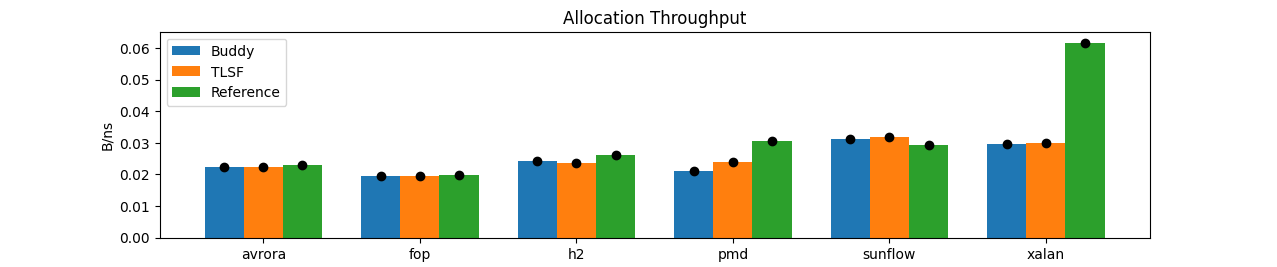
\includegraphics[width=0.6\textwidth]{figures/allocation_throughput.png}
\caption{Barplot showing the allocation throughput of the different allocation strategies when performing relocations.}
\label{fig:allocation-throughput}
\end{figure}

\subsubsection{Free List Initialization Throughput}

In order to measure the cost of searching for the free memory in the fragmented memory of a page, the initialization process of the free-list was introduced. Results shown in Figure~\ref{fig:free-list-initialization} show the throughput you get of initializing the free list. The numbers displayed show us that there is a significant cost to initializing the free list. Important to note here is that the difference in throughput between each of the benchmarks is because of the allocation patterns of the programs, and not a variatation in the performance of the machine running the program. 

\begin{figure}[H]
\centering
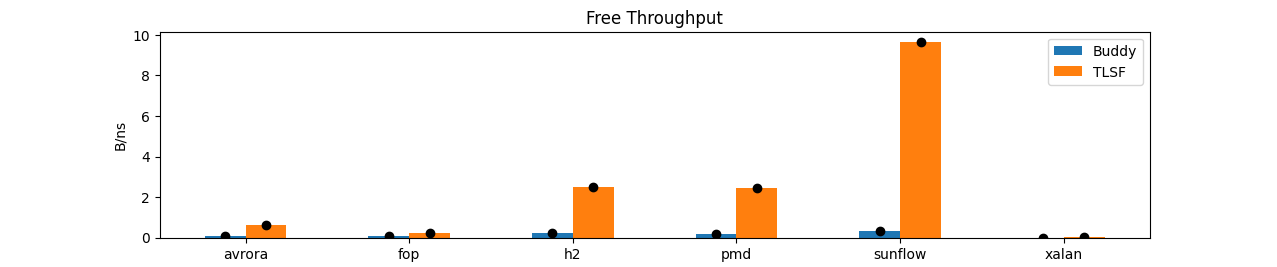
\includegraphics[width=0.6\textwidth]{figures/free_throughput.png}
\caption{Barplot displaying the througput of adding bytes of free memory to the allocator's free-list. The throuhgput is calculated as the amount of bytes found in the fragmented memory, divided by time it took to execute the initialization process.}
\label{fig:free-list-initialization}
\end{figure}

\subsubsection{Fragmentation}
The different allocators demonstrate a significant difference in their ability to makes use of the avaiable memory, displaying some huge variations in how much memory is able to be claimed before an allocation is too large to handle. This is evident from Figure~\ref*{fig:memory-fragmentation}. The plot shows different results for different benchmarking programs, but the TLSF allocator performs significantly better on all benchmarks.

%TODO kanske lägga in samma plot fast med maxreloc_2048 för att få niceigare värden :D 

\begin{figure}[H]
\centering
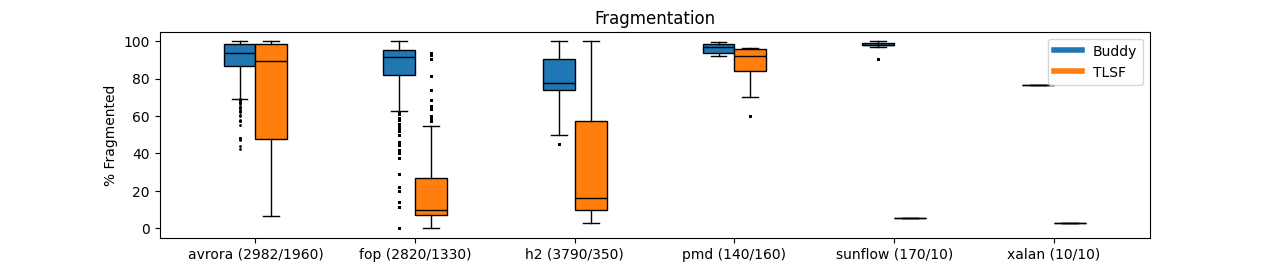
\includegraphics[width=0.6\textwidth]{figures/fl_fragmentation.png}
\caption{Boxplots for each benchmark, and different boxplots for the two implementations measured. Each measured data point is taken from the set of exhausted pages from a full run of the specified benchmark. The fragmentation is measured as the amount of used up bytes, divided by the total amount of bytes available. The numbers displayed by the benchmark name denotes the amount of data points measured for each implementation.}
\label{fig:memory-fragmentation}
\end{figure}

\subsection{Benchmark Performance}
This section evaluates the garbage collector's performance across various benchmarks, focusing on the Java program in its entirety while running with the new implementation of ZGC using free list allocators and comparing that to the reference version of ZGC that the new implementation is built upon.


\subsubsection{Relocation Duration}

Although overall execution time remains stable, there's a marginal increase in time that the garbage collector spends in the relocation phase. In Figure~\ref{fig:relocation-duration}, the relocation duration over multiple runs is shown. It is possible to see a slight upward trend in relocation time for the implementations using free-list relocations. 

\begin{figure}[H]
\centering
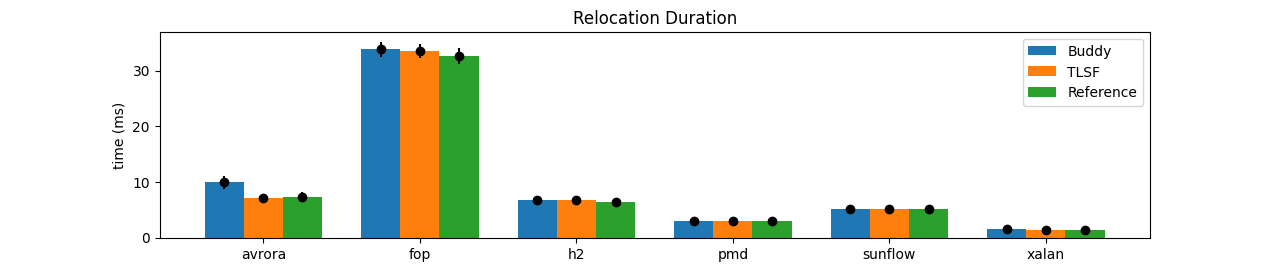
\includegraphics[width=1\textwidth]{figures/relocation.png}
\caption{Barplot showing the average duration that the garbage collector spent in the relocation phase, which is the phase where the reference version is only using bump pointer allocations, while the buddy allocator, and TLSF allocator are making use of a free-list allocation method, as well as resorting to bump pointers when needed.}
\label{fig:relocation-duration}
\end{figure}

\subsubsection{Relocation Set Selection Duration}

This metric shows the time it takes for the garbage collector to select which pages are going to be used for relocation, which is the phase impacted by the initialization of free list memory. In Figure~\ref{fig:set-selection}, a barplot is showing the average time that the different implementations spend in the relocation set selection phase of the garbage collection cycle.

\begin{figure}[H]
\centering
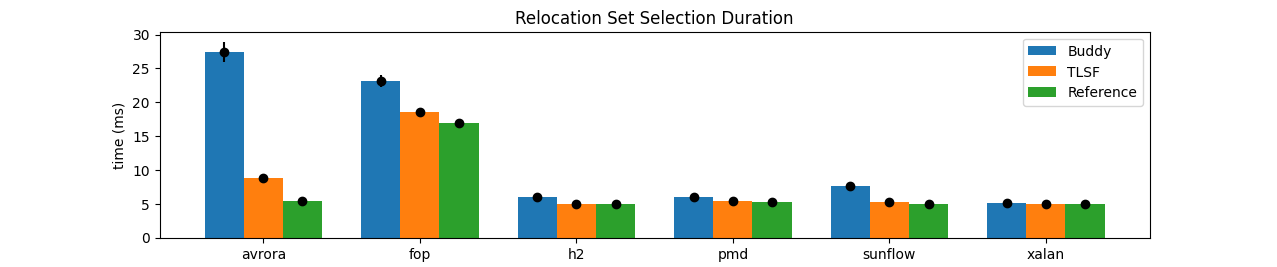
\includegraphics[width=1\textwidth]{figures/set_selection.png}
\caption{Barplot showing the averelocation set Selection Duration Comparison}
\label{fig:set-selection}
\end{figure}


\subsubsection{Throughput}
Through repeated benchmark executions, the execution time remains largely consistent across all implementations, with overlapping confidence intervals. In Figure~\ref{fig:execution-time}, the exeuction times are displayed from running the six different benchmarks for 250 iterations each, comparing the three different implementations.

\begin{figure}[H]
  \centering
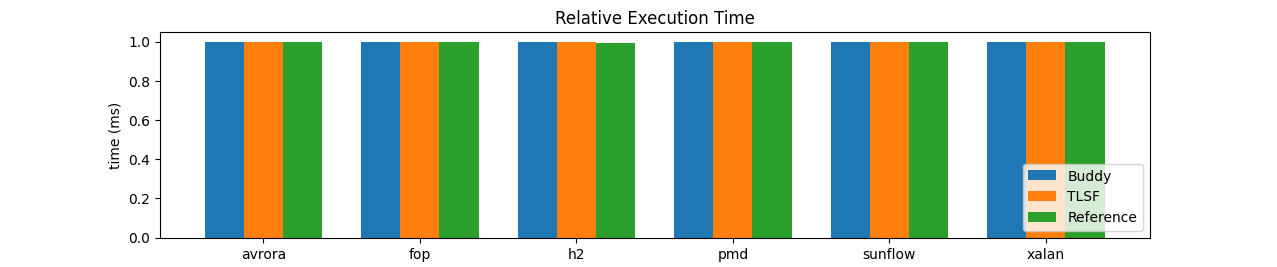
\includegraphics[width=1\textwidth]{figures/execution_time.png}
\caption{Throughput Comparison Across Benchmarks}
\label{fig:exeuction-time}
\end{figure}


\section{Discussion}
\label{sec:discussion}

In this section, the results are discussed from the context of the purpose and goals which were set at the beginning of the project. 

\subsection{Discussing the Results}
The results from this thesis show us that the new type of allocators do not add any significant execution time that decreases the performance of the garbage collector, which is a good sign. Results also show that there is indeed an increased amount of operations being done when the free-list allocator is being used. However, the difference is not large enough to cause any performance issues for the Java program being executed. 

Another good result is that some of the benchmarks used for evaluating displayed good signs of utilizing the fragmented memory for compaction. The benchmark \textit{fop} had an allocation pattern that was able to use very much of the memory that was found in free-list as a location to compact objects into. With an average fragmentation of approximately 10\% when using the TLSF allocator, it shows us that some programs do indeed 

The fact that the execution time does not change is a good result in the sense that the expectation was to have a more computationally heavy allocation method, with the upside of being able to utilize memory more efficiently. The results also prove that the fragmented memory was indeed being utilized. However, these results could suggest that the allocator is not doing as much work as expected. The results from this thesis does not tell us enough about the behaviour of the garbage collector to know if the amount of memory that was saved from using the fragmented memory was enough to cause any increases in performance. Rather, the results hint towards the opposite that the memory saved is not enough to significantly change the behaviour of the program.



%%% Local Variables:
%%% mode: latex
%%% TeX-master: "main"
%%% End:


\section{Conclusions}
\label{sec:conclusions}

%%% Local Variables:
%%% mode: latex
%%% TeX-master: "main"
%%% End:

% talk about how my work can be used to simplify the act of relocating objects into pages that have pinned objects to them
\section{Future Work}
\label{sec:future_work}
The work on the free list allocator has shown that it is possible to integrate a new allocator into the Z Garbage Collector. The results from this thesis has shown that there are indeed differences between using different allocators, and future work could look at which allocator is supposed to be used for certain tasks.

In this thesis, the most promising type of allocator that is to be used for compaction in ZGC is the TLSF allocator, which offered a greater throughput, and also was able reach lower amounts of fragmentation.

%%%% Referenser - SE OCKÅ APPENDIX

% Use one of these:
%   IEEEtranS gives numbered references like [42] sorted by author,
%   IEEEtranSA gives ``alpha''-style references like [Lam81] (also sorted by author)
\bibliographystyle{IEEEtranS}
%\bibliographystyle{IEEEtranSA}

% Here comes the bibliography/references.
% För att göra inställningar för IEEEtranS/SA kan man använda ett speciellt bibtex-entry @IEEEtranBSTCTL,
% se IEEEtran/bibtex/IEEEtran_bst_HOWTO.pdf, avsnitt VII, eller sista biten av IEEEtran/bibtex/IEEEexample.bib.
\bibliography{bibconfig,refs}
%\bibliography{refs}

\newpage
\appendix %%%% markerar att resten är appendixar
%%%% I er egen version, ta bort allt nedan (utom \end{document})

%%% Local Variables:
%%% mode: latex
%%% TeX-master: "main"
%%% End:


% Om ni har ett index
\makeatletter
\renewenvironment{theindex}
{\if@twocolumn
    \@restonecolfalse
  \else
    \@restonecoltrue
  \fi
  \twocolumn[\section{\indexname}]%
  \@mkboth{\MakeUppercase\indexname}%
  {\MakeUppercase\indexname}%
  \thispagestyle{plain}\parindent\z@
  \parskip\z@ \@plus .3\p@\relax
  \columnseprule \z@
  \columnsep 35\p@
  \let\item\@idxitem}
{\if@restonecol\onecolumn\else\clearpage\fi}
\makeatother
\printindex
\end{document}
